%%%%%%%%%%%%%%%%%%%%%%%%%%%%%%%%%%%%%%%%%%%%%%%%%%%%%%%%%%%%%%%%%%%%%%%%%%%%
%% Trim Size : 11in x 8.5in
%% Text Area : 9.6in (include Runningheads) x 7in
%% ws-jai.tex, 26 April 2012
%% Tex file to use with ws-jai.cls written in Latex2E.
%% The content, structure, format and layout of this style file is the
%% property of World Scientific Publishing Co. Pte. Ltd.
%%%%%%%%%%%%%%%%%%%%%%%%%%%%%%%%%%%%%%%%%%%%%%%%%%%%%%%%%%%%%%%%%%%%%%%%%%%%
%%

%\documentclass[draft]{ws-jai}
\documentclass{ws-jai}
\usepackage[flushleft]{threeparttable}
\begin{document}

\catchline{}{}{}{}{} % Publisher's Area please ignore

\markboth{Bunch O people}{Analysis of robustness of BINGO optics.}

\title{Analysis of Robustness of BINGO optics.}

\author{First Author$^{2}$, Second Author$^{3}$, Third Author$^{3}$ and Fourth Author$^{4}$}

\address{
$^{2}$Department, University Name, City, State ZIP/Zone, Country, fauthor@university.com\\
$^{3}$Group, Company, Address, City, State ZIP/Zone, Country\\
$^{4}$Group, Company, Address, City, State ZIP/Zone, Country, fauthor@company.com
}

\maketitle

\corres{$^{2}$Corresponding author.}

\begin{history}
\received{(to be inserted by publisher)};
\revised{(to be inserted by publisher)};
\accepted{(to be inserted by publisher)};
\end{history}

\begin{abstract}
The BINGO (Baryon Acoustic Oscillations [BAO] from Integrated Neutral Gas Observations) project is a single dish transit telescope aiming to do 21-cm Intensity Mapping observations, located in northeast of Brazil. Deviations from feed or mirror positions would lead to loss in efficiency. In this paper we analyze the effect of possible geometric deformations of the telescope optics and establish constraints to be met in the construction work. We found that all parts of the telescope should be positioned with a precision of a few centimeters, representing a typical accuracy of 0.1\%, which is quite feasible to do with the metallic structure design that is being implemented.
\end{abstract}

\keywords{Keyword 1; keyword 2; keyword 3.}

\section{The Main Text}
\noindent The BINGO (Baryon Acoustic Oscillations [BAO] from Integrated Neutral Gas Observations) project is a single dish transit telescope aiming to do 21-cm Intensity Mapping observations, located in northeast of Brazil. \ref{bingoI, bingoII}

BINGO telescope main science case is very demanding. HI brigthness temperature is $10^{-5}$ times the typical astrophysical foregrounds and construct of a succesful data cleaning pipeline implies very good sensitivity, achieved by low ellipticity, low cross-polarization and low side-lobes.

The optics of the telescope is of cross-dragone type, consisting of an off-axis paraboloid coupled with an off-axis hyperboloid, feed is in a very large focal plane, laterally placed. BINGO project will have 28 feeds populating the focal plane and the detailed scheme of the focal plane is described in \ref{bingoIII}. In this work we consider the nominal optics with a central horn, as depicted in \ref{fig:bingo_optics}.

\begin{figure}
\begin{center}
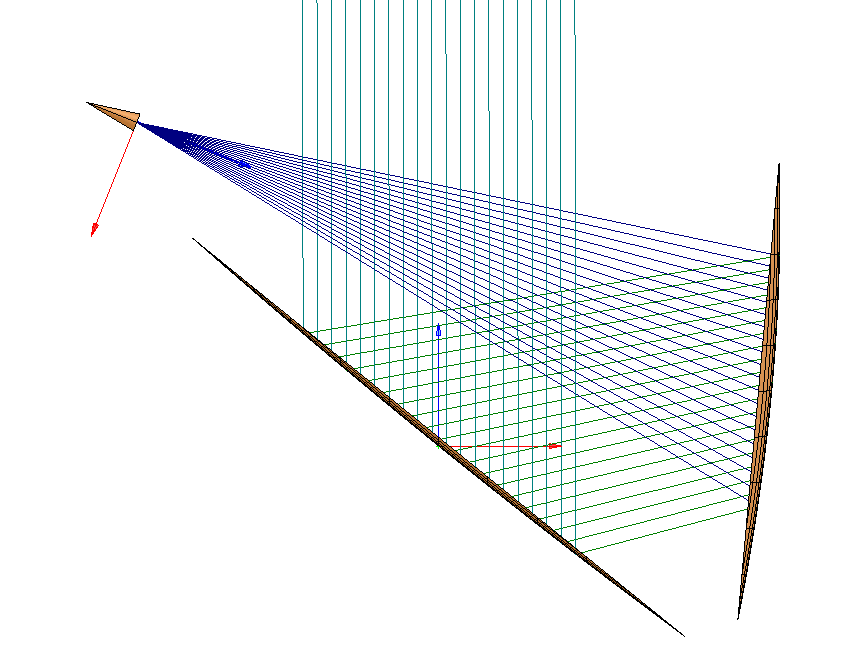
\includegraphics[width=7in]{./figs/GRASP_VIEW}
\end{center}
\caption{BINGO optics.}
\label{fig:bingo_optics}
\end{figure}


BINGO telescope will consist of a metallic structure constructued similarly to FAST (Five hundred meter Aperture Spherical radio Telescope), the world's largest telescope in operation in Guizhou Province, in southwest China \ref{fast01}.

Accurate positioning of the structures during building phase is of utmost importance, and is relevant to consider which are the physical constraints to be met.

In the following work we analyze three dimensional motions of feed and secondary in order to establish criteria for accuracy constraints in building work.

\section{BINGO geometry}

BINGO geometry may be described using three coordinate systems. A global coordinate system where the main primary (paraboloid) mirror surface is defined (this coordinate system is not shown in \ref{fig:bingo_optics}). Also we have the feed coordinate system, depicted at the tip of the feed in \ref{fig:bingo_optics}) and, finally, a coordinate system where the secondary (hyperboloid) surface mirror is defined, depicted at the center of the figure \ref{fig:bingo_optics}).

For all coordinate systems, blue axis indicates the $z$ direction and red axis indicates $x$ direction. The $y$ coordinate is always given by $\hat z \times \hat x$ with the usual orientation.

As a rigid body, the feed has 6 degrees of freedom of motion, three translations and three rotations. Since the feed is oriented with its symettry axis in the $z$ direction, rotations around this axis may contribute with polarization diferences due to any assymetry inthe beam, however, bingo beam is highly symmetric and we are going to consider only simulations with a perfect gaussian beam for simplicity, which means that rotations of the feed around this axis should not be considered.


\section{Metrics for Optical Performance}

Any geometric distortion or misplacement of telescope structure may impact in the characteristics of the Beam, which may usually be considered as impacting the effective area of the telescope \ref{baars}. Calculating these efficiencies require integrating the near fields in the aperture.

In this work we are going to consider only one parameter directly related to an aperture integral, the spillover of the main mirror. This may be obtained integrating the poyinting vector in the aperture:

\begin{eqnarray}
\vec S &=& \frac{1}{2} \mathrm{Re} \vec E \times \vec H\\
W &=& \iint_A d\vec a \cdot \vec S \\
\eta_{spillover_{dB}} &=& 10 \log_{10} \frac{4\pi}{W},
\end{eqnarray}

where the integral is over the aperture.

Several other parameters may be obtained with the far fields and the beam pattern. In this work we consider the directivity as the relevant parameter:

\begin{eqnarray}
\eta_{D_{dB}} = 10 \log_{10} \frac{4 \pi \Vert E^2\Vert_{max}}{\iint \Vert E^2\Vert d\Omega},
\end{eqnarray}

where the electric field is the far-field and the integral is over the solid angle. We consider azimuthal symmetry and perform the integration in $\theta$ only.

We considerer the fractional change of each of thes metrics and set the goal that the fractional change should be less than 1 percent for each metric. We define the fracional change of any of the metrics as

\begin{equation}
\delta \eta = \frac{\vert \eta - \eta_0\vert}{\eta_0,}
\end{equation}

where $\eta_0$ is the value obtained with the nominal parameters of the telescope, therefore it's the undeformed value.

\section{Simulations}

\subsection{Methodology}

We implement the geometry of the telescope with one central horn in TICRA GRASP software for eletromagnetic simulations, and we set a job to calculate the beam pattern in the far field, considering the feed iluminating the secondary and obtaining the resultant field in the main mirror, including its electric response. GRASP simulations is very straighforward and provides both the spill over and the beam pattern.

An external python script produces the changes in the geometry and programatically run the EM simulation, calculating the metrics we are interested in.


\subsection{Effects of Feed Positioning Error}

\begin{figure}
\begin{center}
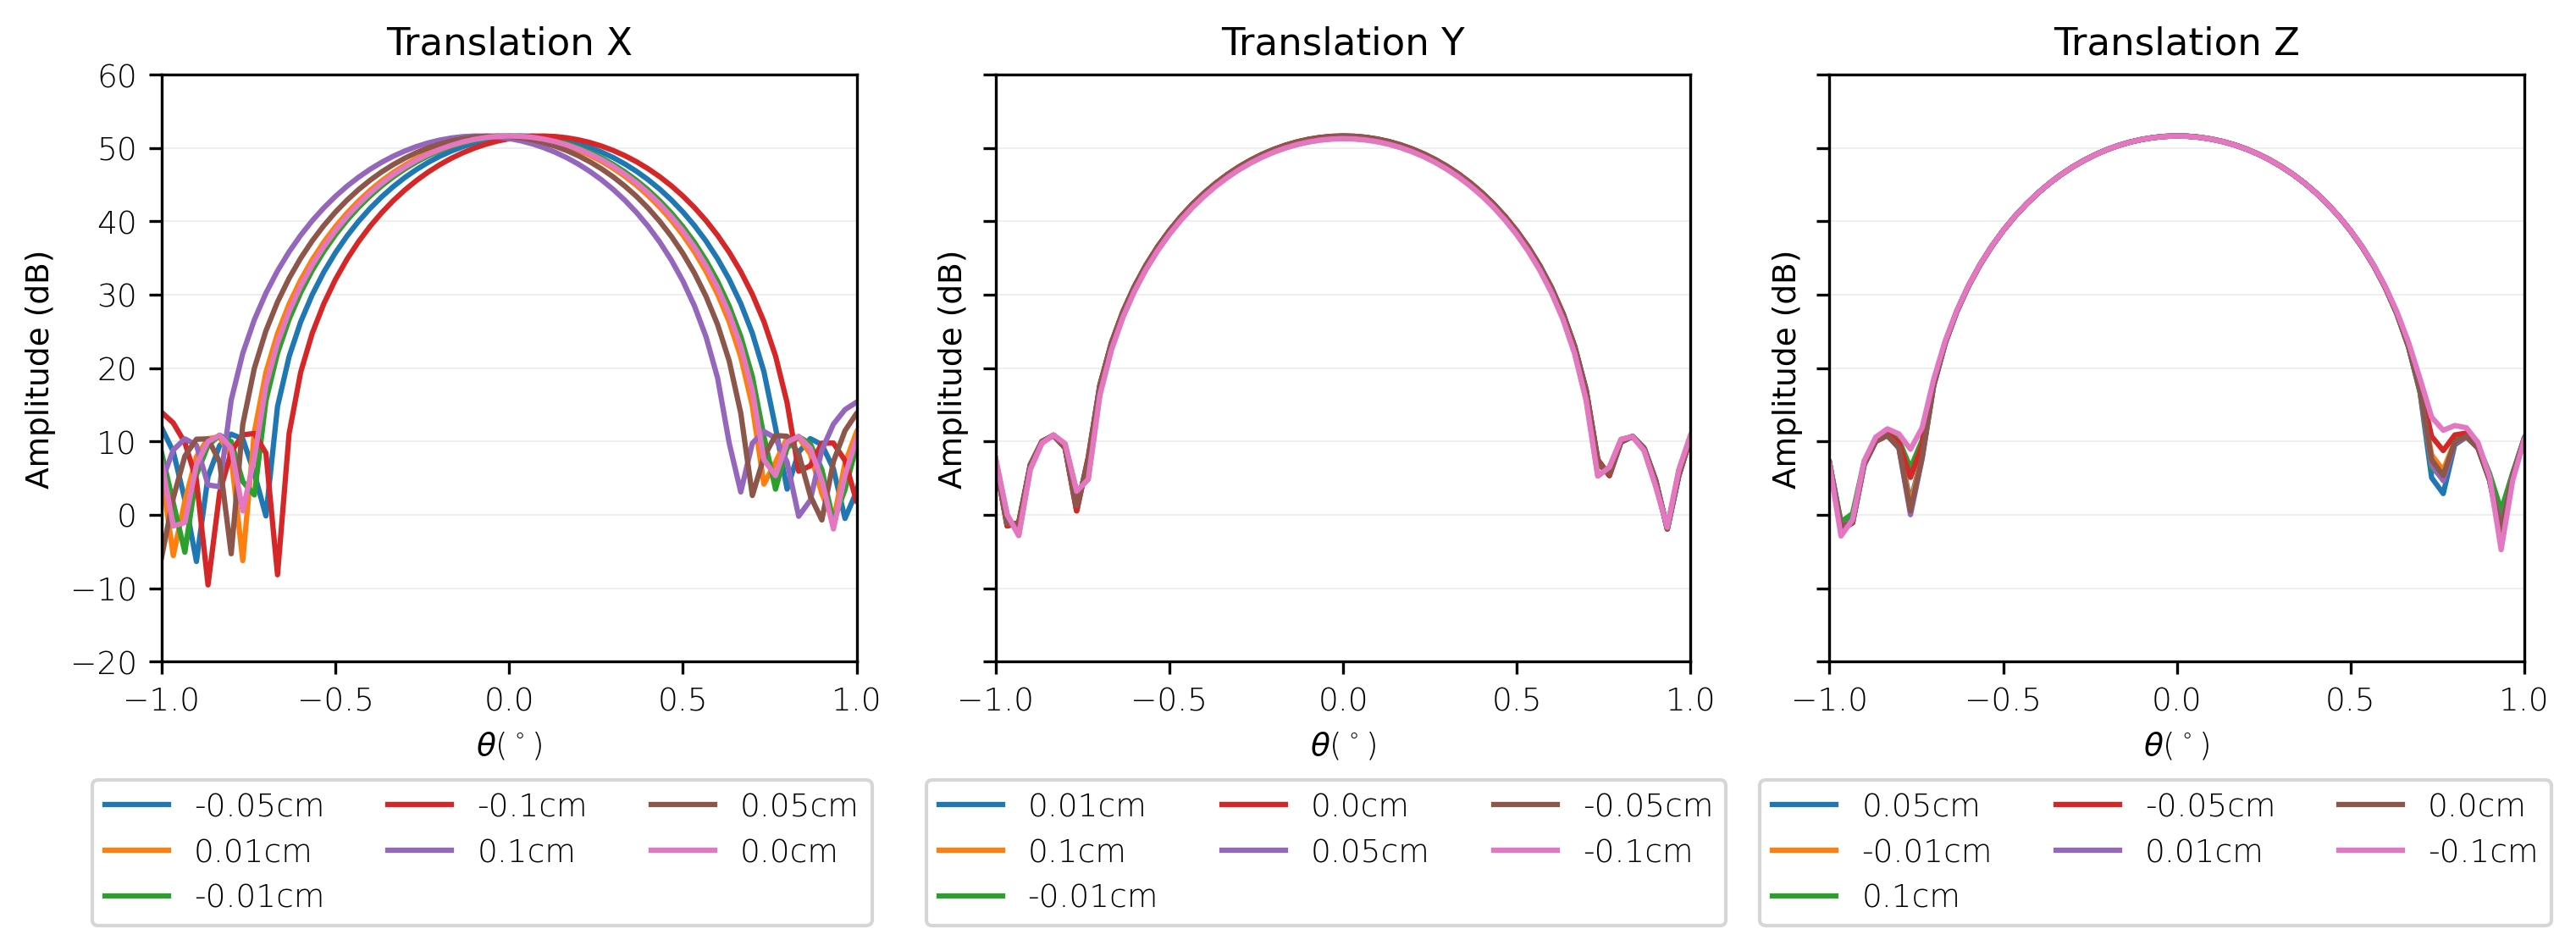
\includegraphics[width=7in]{figs/01_feed_trans_XYZ}
\end{center}
\caption{Beam pattern obtained translating the feed in the indicated directions.}
\label{fig:feed_trans_XYZ}
\end{figure}

\begin{figure}
\begin{center}
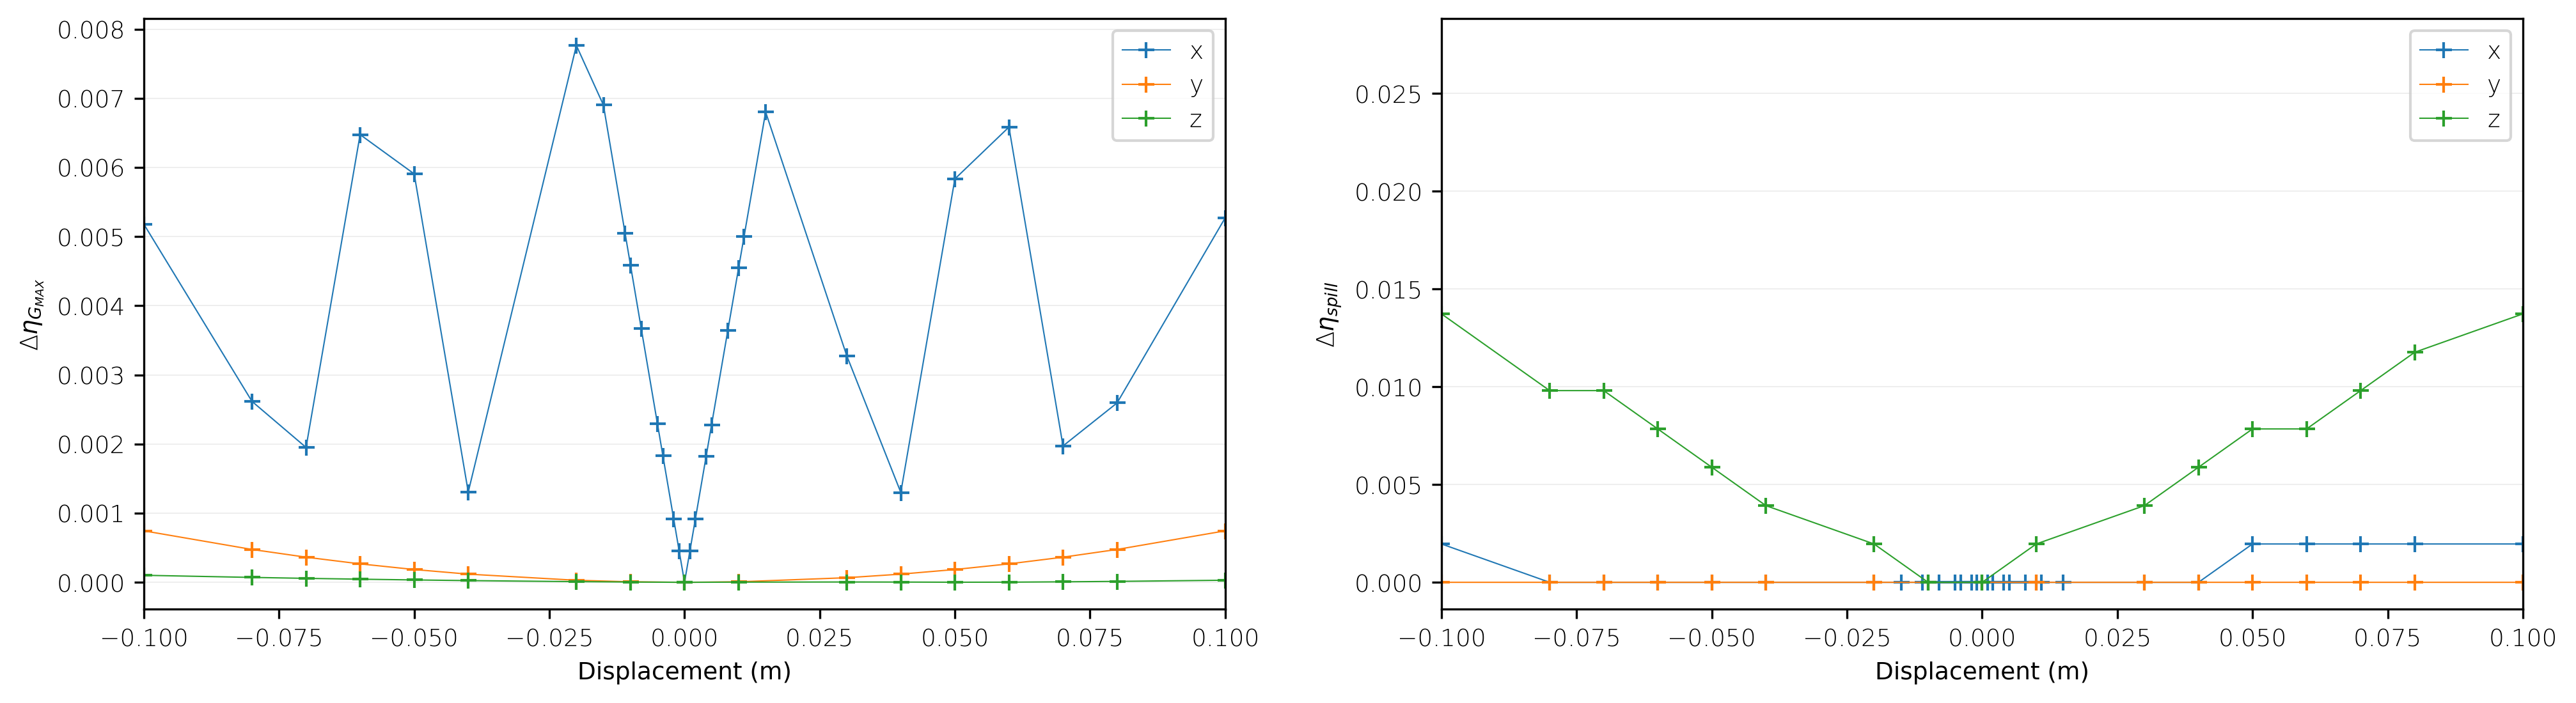
\includegraphics[width=7in]{figs/02_feed_trans_XYZ_bounds}
\end{center}
\caption{Each line indicates the fractional change in directiviy (left) and spillover (right) for translations of the feed in the three orientations by the amounts indicated in the x-axis of the plots.}
\label{fig:feed_trans_XYZ_bounds}
\end{figure}

\begin{figure}
\begin{center}
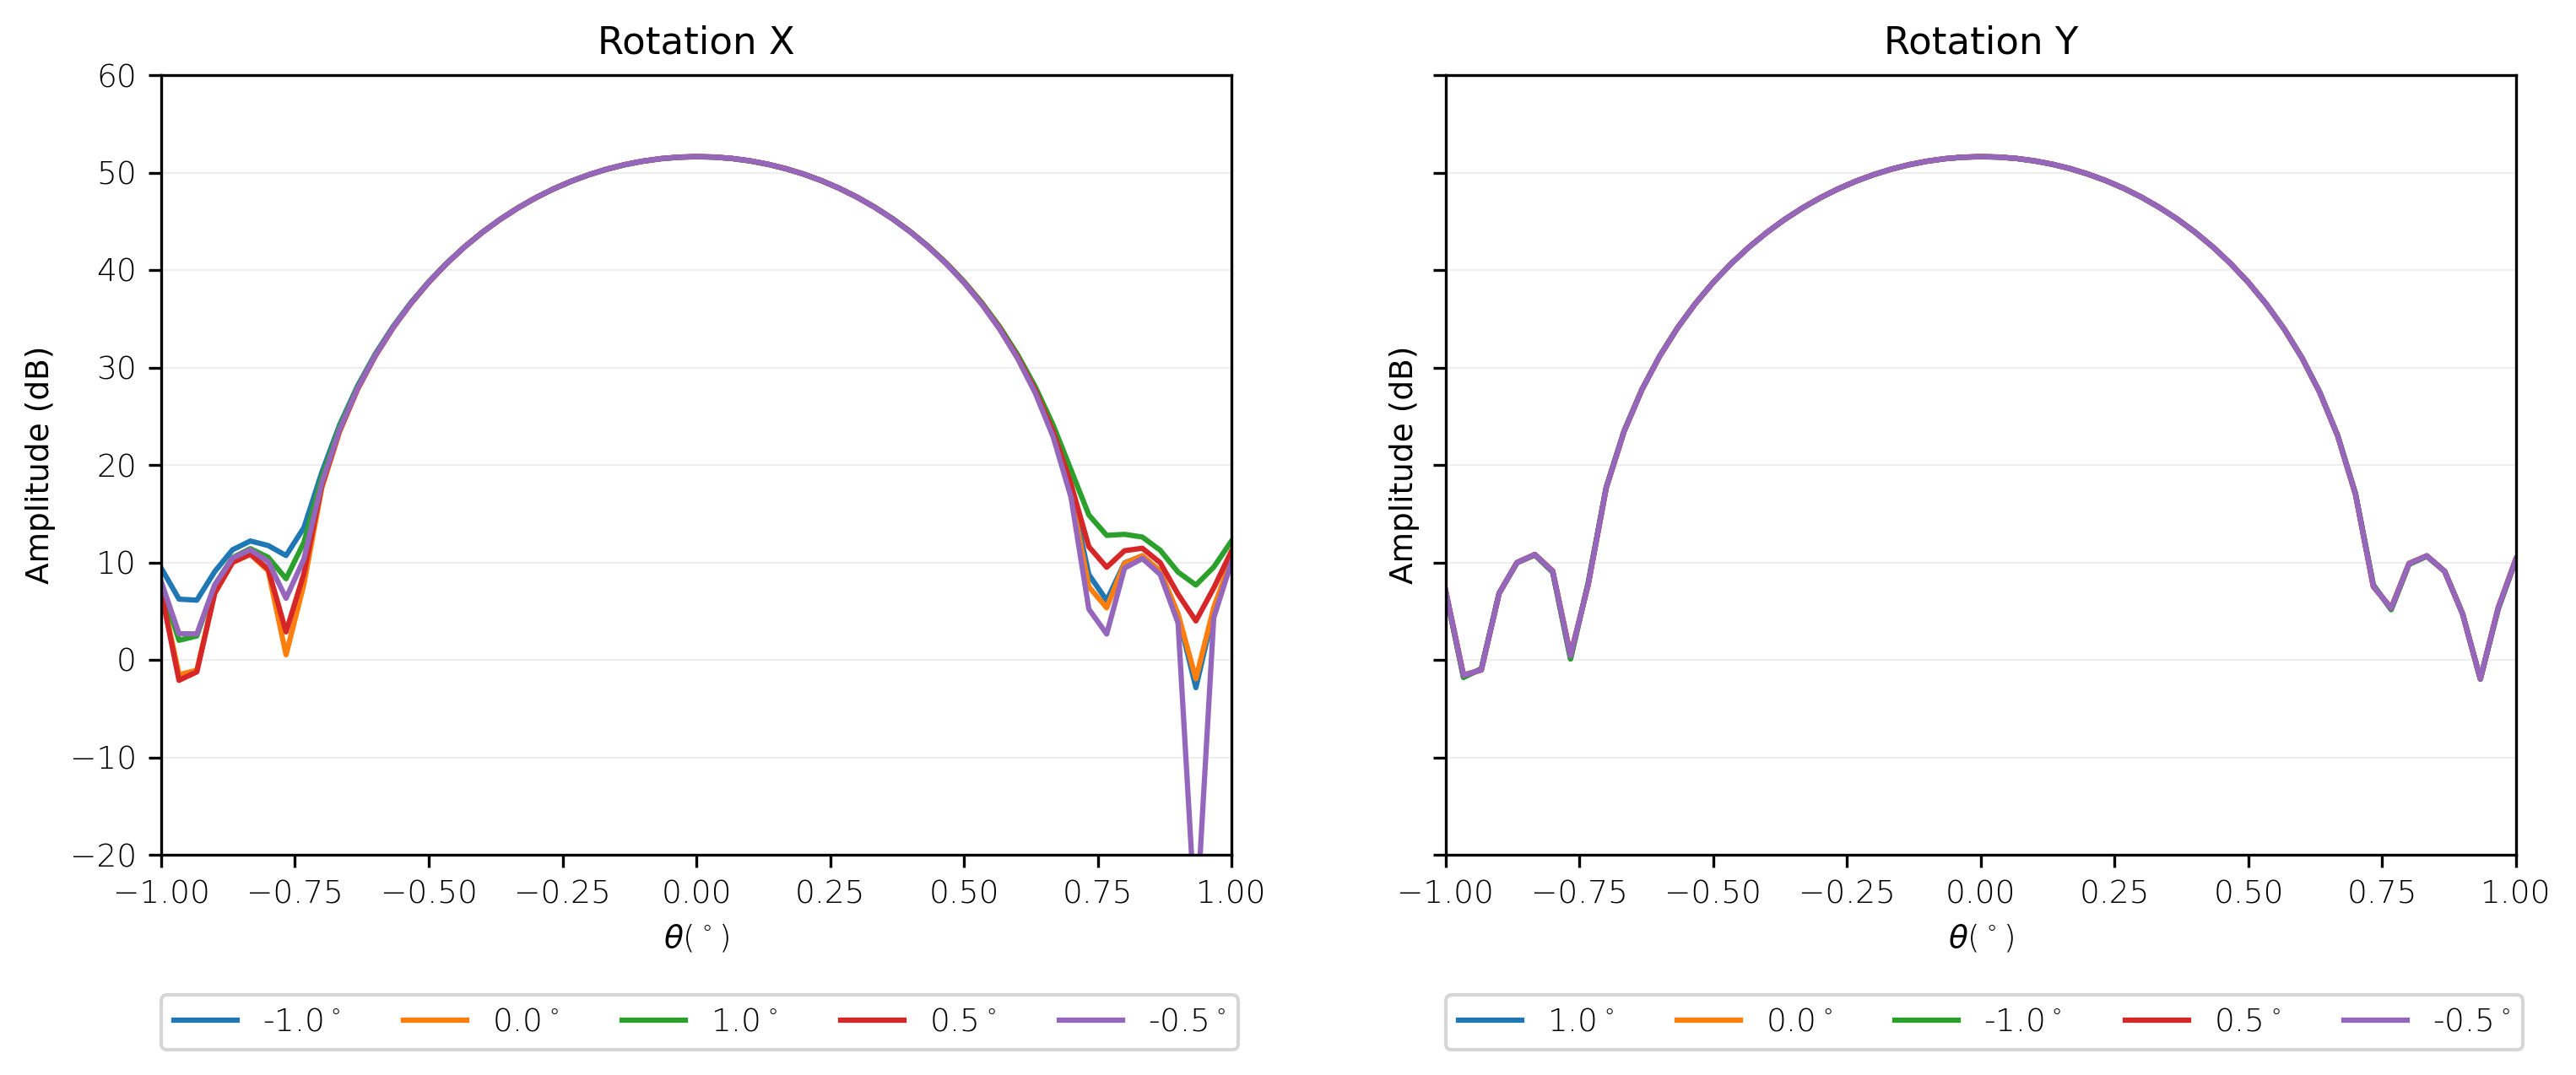
\includegraphics[width=7in]{figs/03_feed_rot_XY}
\end{center}
\caption{Beam pattern obtained rotating the feed in the indicated directions.}
\label{fig:feed_rot_XY}
\end{figure}

\begin{figure}
\begin{center}
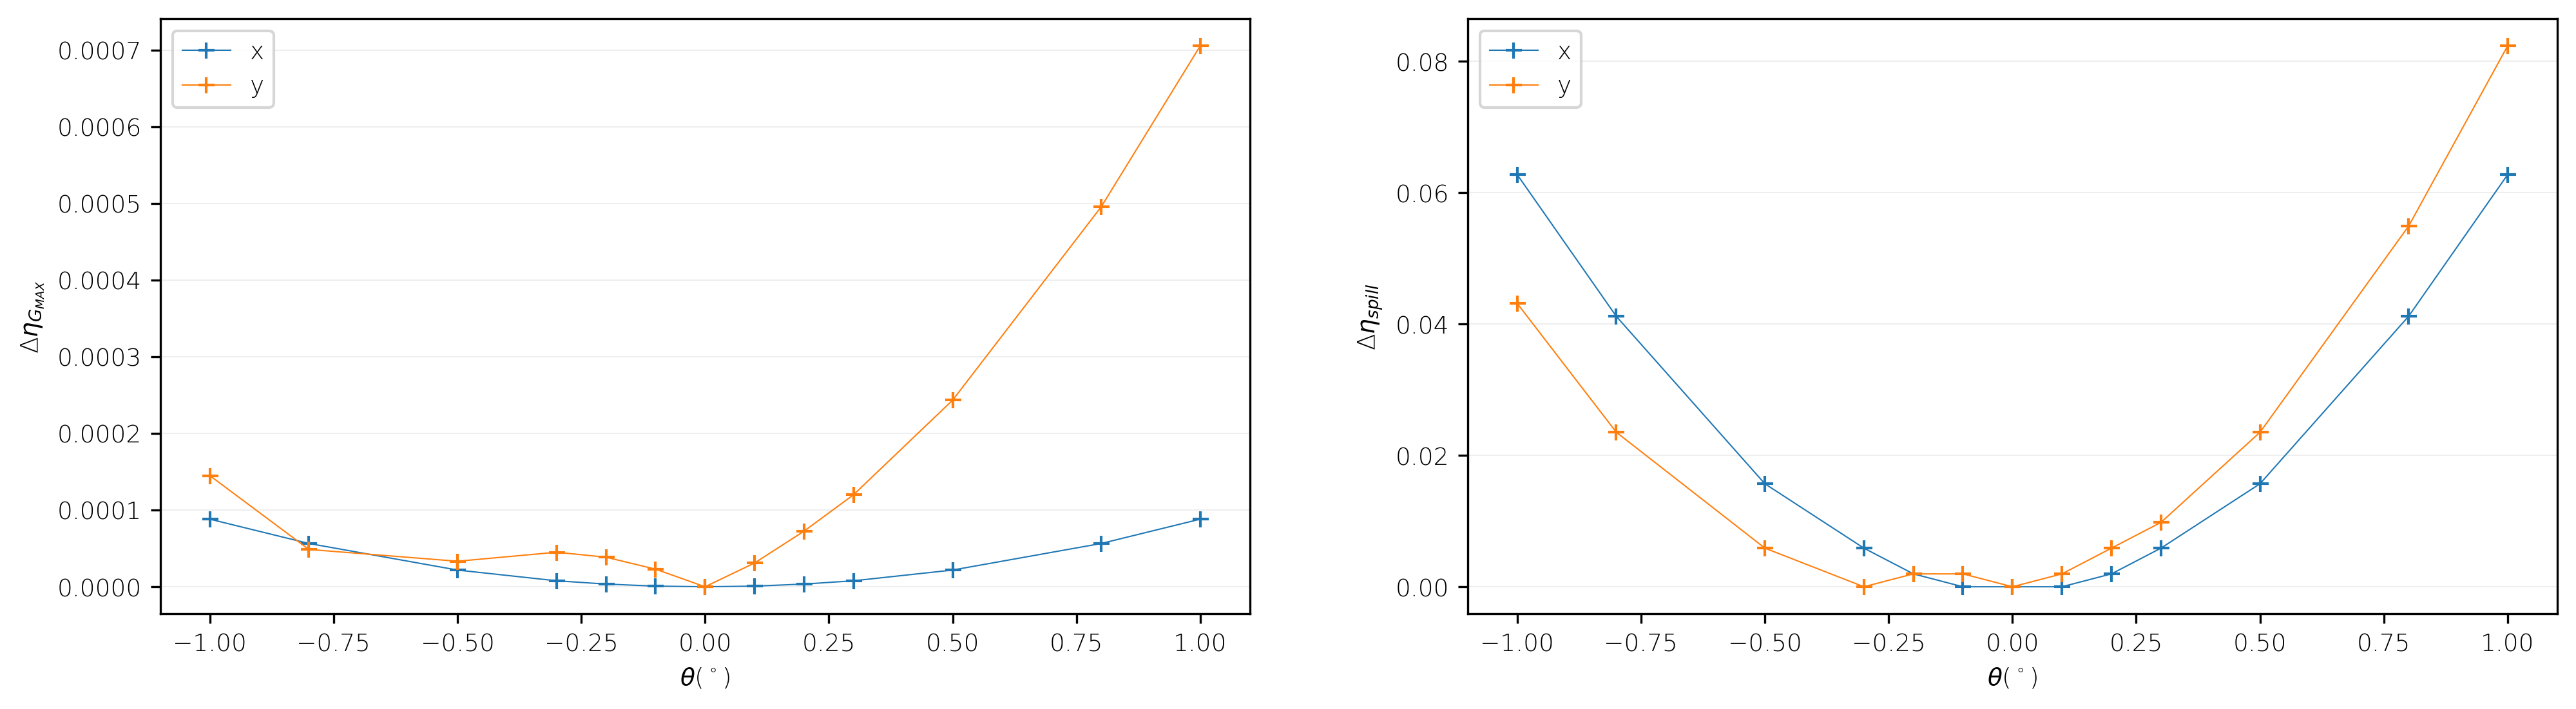
\includegraphics[width=7in]{figs/04_feed_rot_XY_bounds}
\end{center}
\caption{Each line indicates the fractional change in directiviy (left) and spillover (right) for rotations of the feed in the two orientations by the amounts indicated in the x-axis of the plots.}
\label{fig:feed_rot_XY_bounds}
\end{figure}

\subsection{Effects of Secondary Positioning Error}

\begin{figure}
\begin{center}
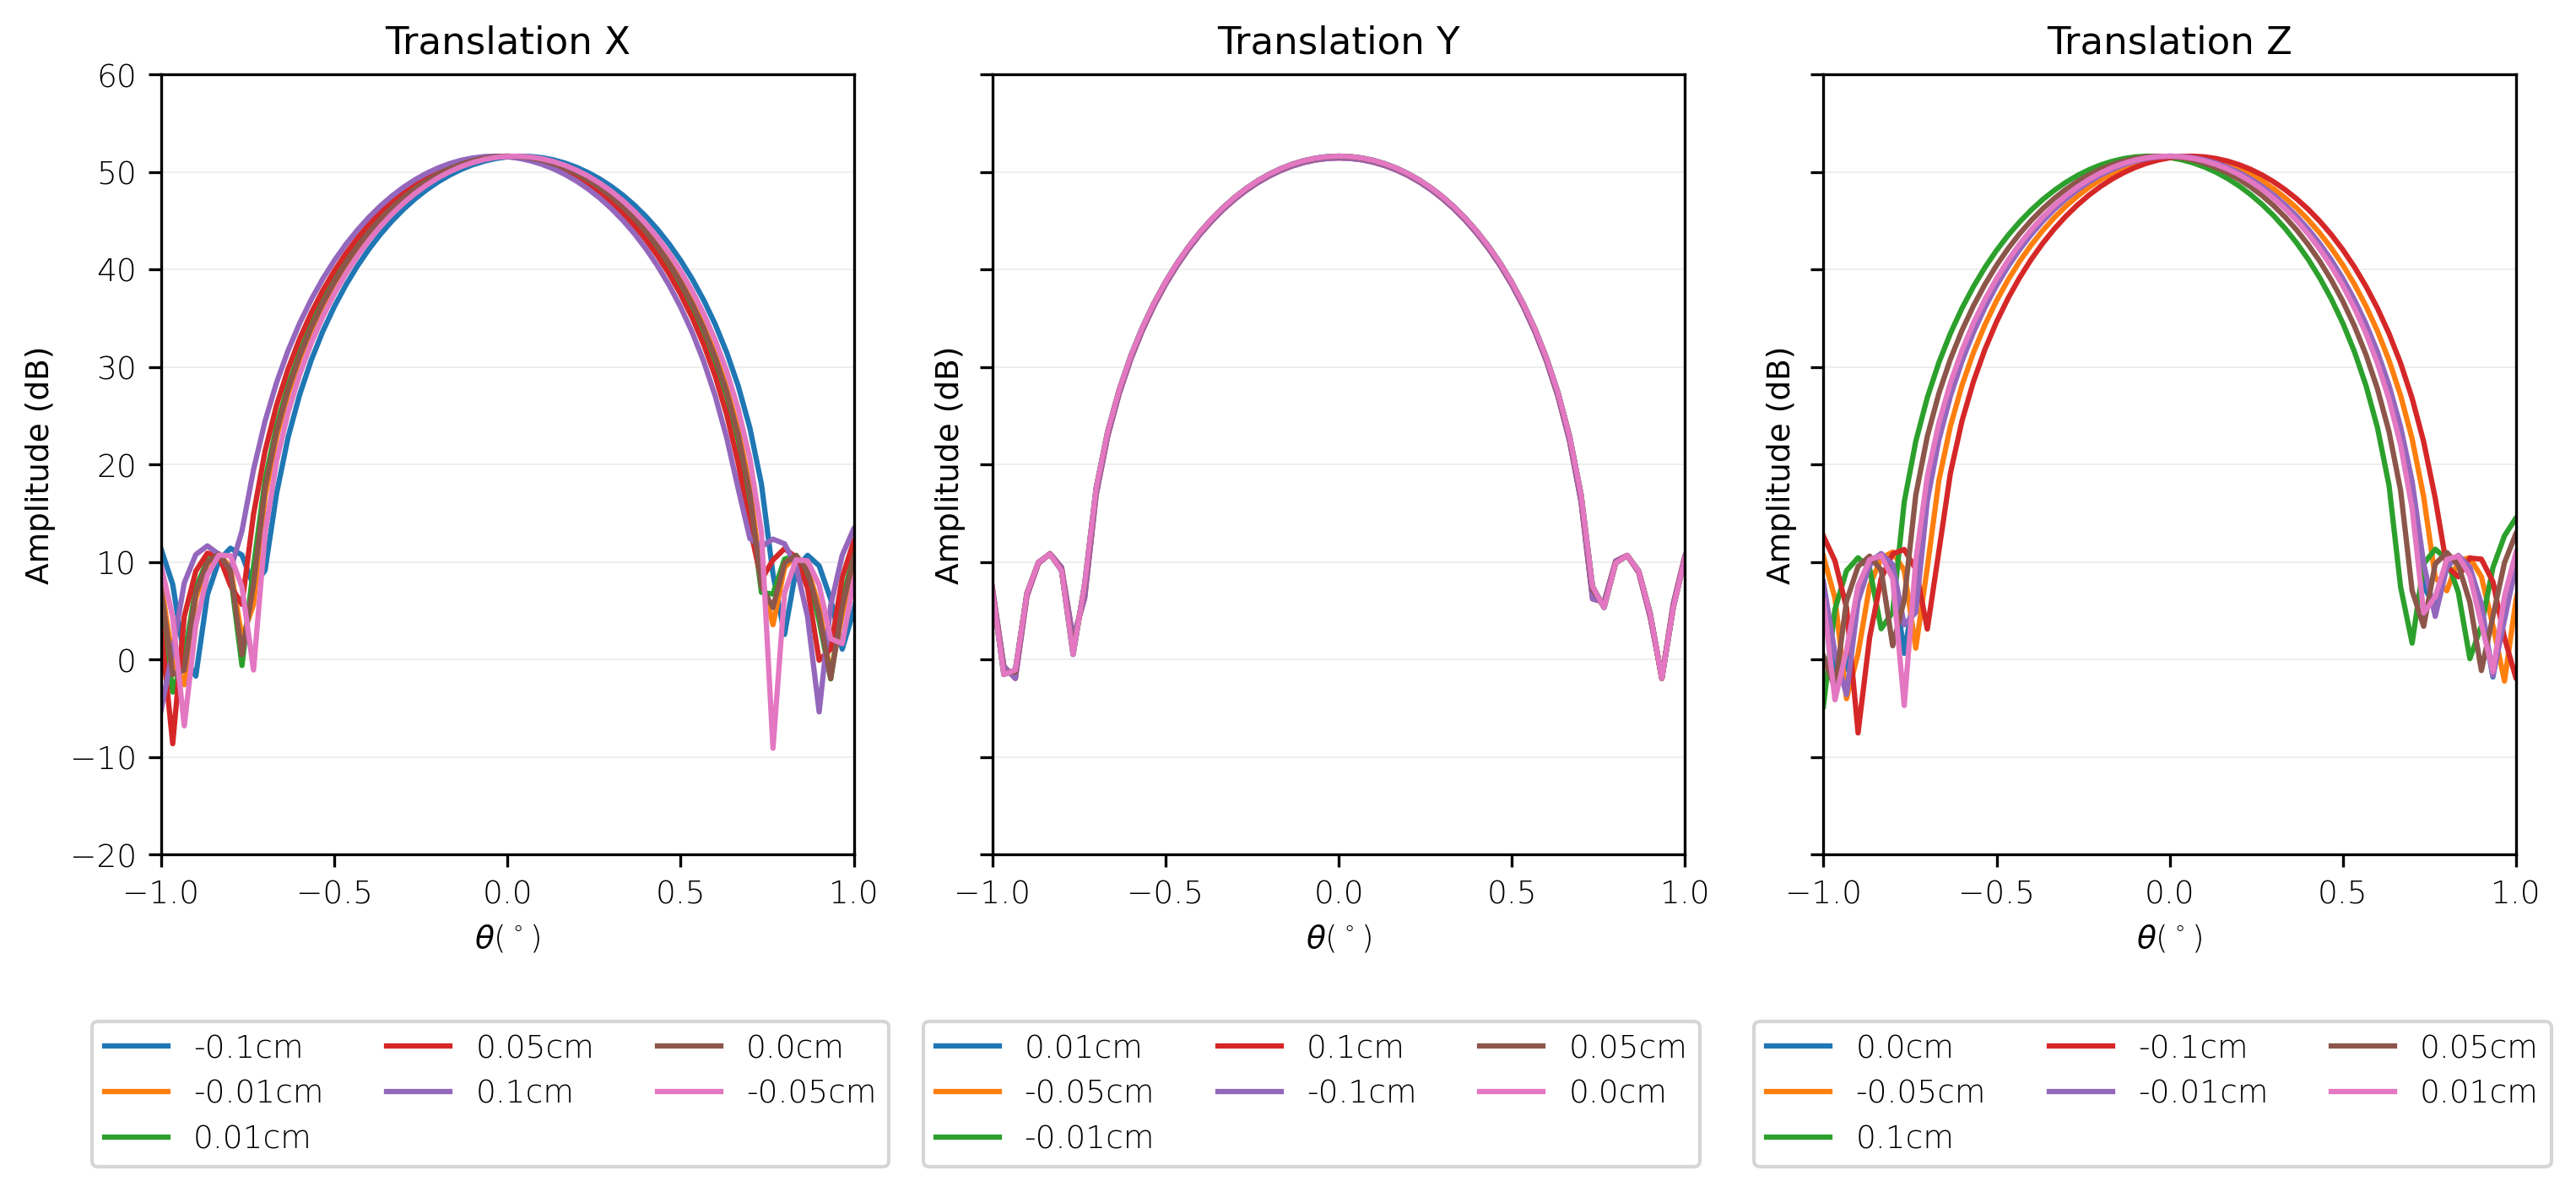
\includegraphics[width=7in]{figs/05_sec_trans_XYZ}
\end{center}
\caption{Beam pattern obtained translating the secondary mirror the indicated directions.}
\label{fig:sec_trans_XYZ}
\end{figure}

\begin{figure}
\begin{center}
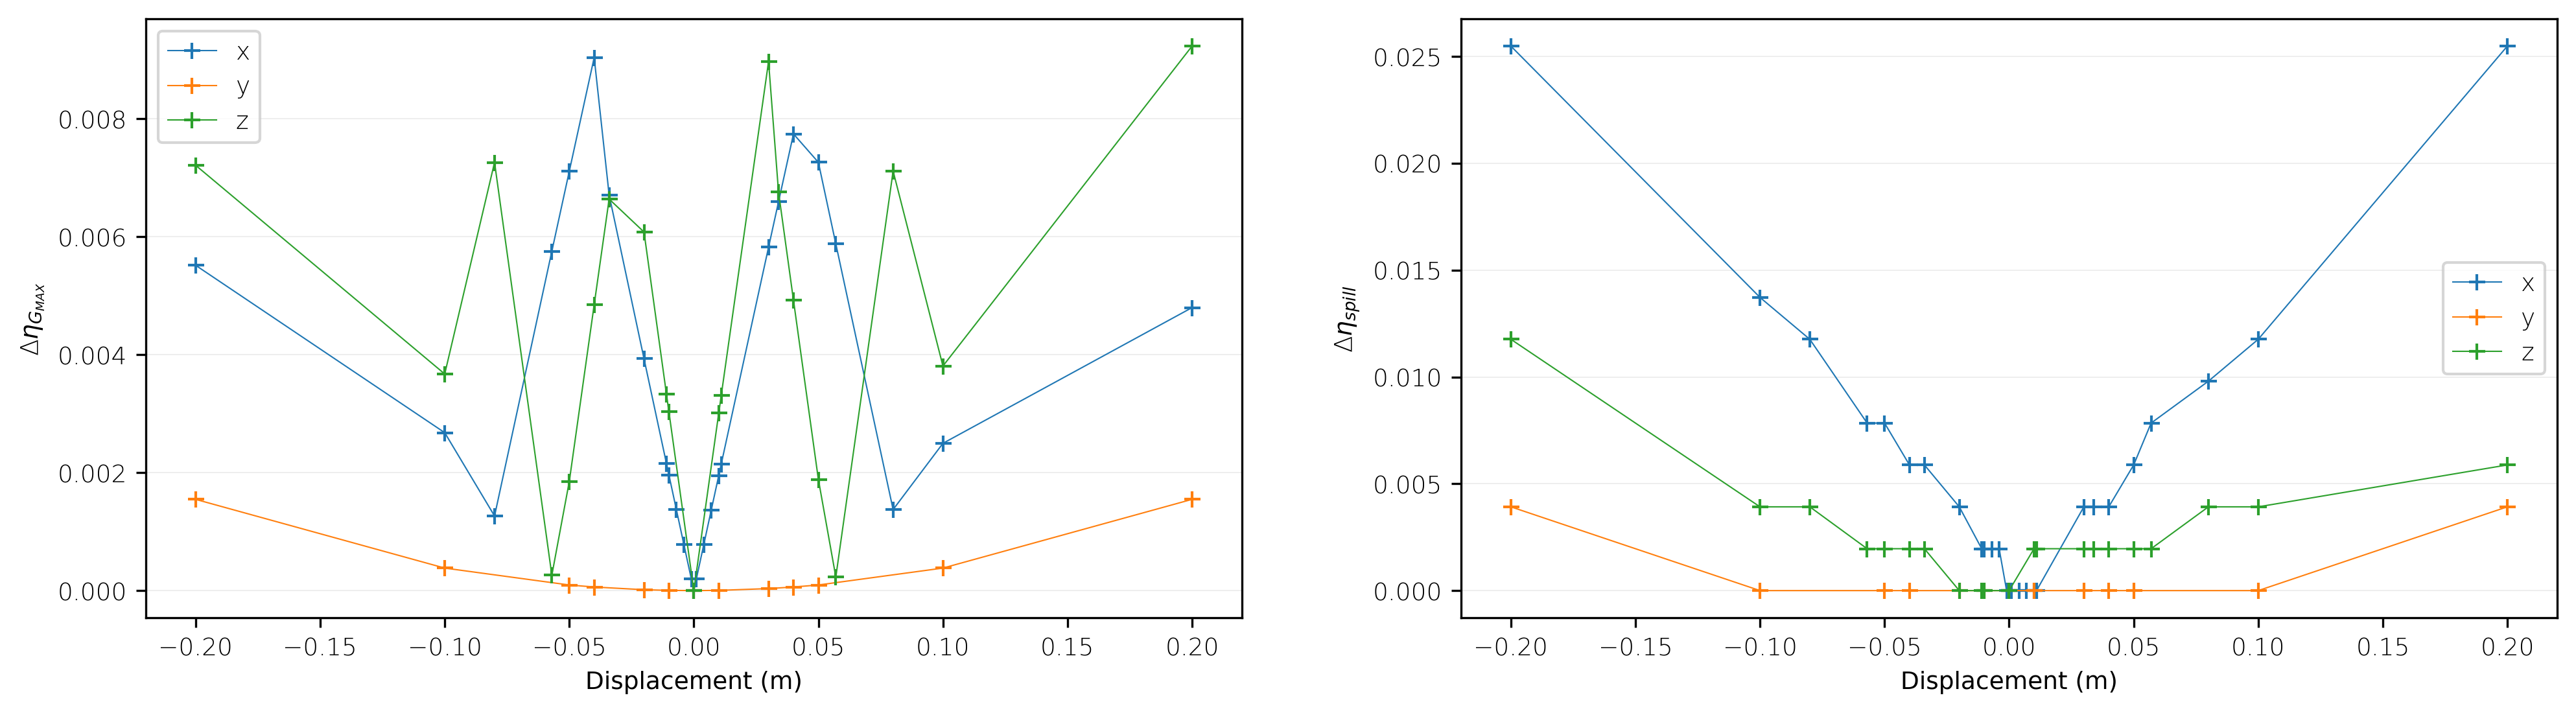
\includegraphics[width=7in]{figs/06_sec_trans_XYZ_bounds}
\end{center}
\caption{Each line indicates the fractional change in directiviy (left) and spillover (right) for translations of the secondary mirror in the three orientations by the amounts indicated in the x-axis of the plots.}
\label{fig:sec_trans_XYZ_bounds}
\end{figure}

\subsection{Accuracy constraints}

In all cases, spill over was the with bigger fraccional changes, setting the upper limits for the variation of positions.

\begin{wstable}[h]
\caption{limits for accuracy.}
\begin{tabular}{lr}
\toprule
Dimension & bound \\
\toprule
$\Delta X_{feed}$  & \hphantom{0}$< 0.20$ m \\
$\Delta Y_{feed}$  & \hphantom{0} $< 0.20$ m \\
$\Delta Z_{feed}$  & \hphantom{0} $< 0.07$ m \\
$\Delta \theta_{feed_x}$  & \hphantom{0}$< 0.30^\circ$  \\
$\Delta \theta_{feed_y}$  & \hphantom{0}$< 0.30^\circ$  \\
$\Delta X_{sec}$  & \hphantom{0} $< 0.08$ m \\
$\Delta Y_{sec}$  & \hphantom{0} $< 0.20$ m \\
$\Delta Z_{sec}$  & \hphantom{0} $< 0.20$ m \\ \botrule
\end{tabular}
\label{aba:tbl1}
\end{wstable}


\section{Conclusions and Discussion}



\section*{Note Added}
A note can be added before Acknowledgments.

\section*{Acknowledgments}
This part should come before References. Funding information may also be included here.


\bibliographystyle{ws-jai}

\bibliography{sample}
\end{document}
